%-------------------------------------------------------
\section{Zero lower bound and Policy responses}
%-------------------------------------------------------

\begin{frame}

\begin{center}
{\LARGE Zero lower bound and Policy responses}
\end{center}

\end{frame}

%-------------------------------------------------------

%-------------------------------------------------------
	
\begin{frame}{Zero lower bound}

Shocks and long term trends can drive the $r_{t}$ desired by the CB below zero
\begin{itemize}
\item	Perhaps easiest to think about demand-side shocks/trends
\item	Remember our simple models where a lower interest rate was required if the desire to save was strong (i.e. current demand is relatively low)
\end{itemize}

\vspace{3mm}
Why might people not be able or want to borrow so much at a given $r_{t}$?
\begin{itemize}
\item	Aging populations and longer life spans (saving for retirement)
\item	`Savings glut' from Asian central banks accumulating Treasuries
\item	Banks tightening lending $\Rightarrow$ a given $r_{t}$ has a larger spread on top
\item	Flight to safety and/or post crisis regulation $\Rightarrow$ demand for safe assets 
\item	Slower growth and secular stagnation
\end{itemize}

\end{frame}

%-------------------------------------------------------

%-------------------------------------------------------
	
\begin{frame}{Falling real rates}

Use the intuition of an Euler equation (ignore risk) under CRRA felicity:
\begin{eqnarray*}
1 &=& 	\beta \frac{Z_{t+1}}{Z_{t}} R_{t} \frac{U_{c,t+1}}{U_{c,t}} \\
	&=& \beta \frac{Z_{t+1}}{Z_{t}} R_{t} \left( \frac{C_{t+1}}{C_{t}} \right)^{-\sigma}
\end{eqnarray*}

Rearrange to obtain
\[
R_{t} = \left(\frac{C_{t+1}}{C_{t}}\right)^{\sigma} \frac{Z_{t+1}}{Z_{t}} \beta^{-1}
\]

And in logs
\[
r_{t} = \sigma \Delta c_{t+1} - \Delta z_{t+1} + \rho
\]
recalling $\rho \equiv -\log{\beta}$ (and log of a ratio is difference of logs)

\end{frame}

%-------------------------------------------------------

%-------------------------------------------------------
	
\begin{frame}{Falling real rates}

What follows isn't a complete G.E. argument - a bit loose - but useful for intuition\ldots

\end{frame}

%-------------------------------------------------------

%-------------------------------------------------------
	
\begin{frame}{Falling real rates - short run}

\[
r_{t} = \sigma \Delta c_{t+1} - \Delta z_{t+1} + \rho
\]
Households anticipate a future contraction driving consumption down
\begin{itemize}
\item	$\Delta c_{t+1}\downarrow$
\end{itemize}
\[
r_{t} = \sigma \Delta c_{t+1} - \Delta z_{t+1} + \rho
\]
Households' `confidence' $\downarrow$ and want to build up `rainy day' fund
\begin{itemize}
\item	Reinterpret $Z_{t}$ as capturing temporary changes precaution
\item	$\Delta z_{t+1} \uparrow$ (from $z_{t}\downarrow$) like becoming relatively patient now
%\item	Like temporarily higher $\beta$ (lower $\rho$)
\end{itemize}
\vspace{1.5mm}
\[
r_{t}^{HH} \equiv r_{t} + \Delta z_{t+1} = \sigma \Delta c_{t+1} + \rho
\]
Households borrow at $r_{t}$ \textit{plus a spread}
\begin{itemize}
\item	Reinterpret $Z_{t}$ as capturing banks' willingness to lend (lower spread)
\item	$\Delta z_{t+1} \uparrow$ (from $z_{t}\downarrow$) reflects financial shock damaging banks
%\item	Plot equation in $(r_{t},\Delta c_{t+1})$ space and play with $\Delta z_{t+1}$
\end{itemize}

\end{frame}

%-------------------------------------------------------

%-------------------------------------------------------
	
\begin{frame}{Falling real rates - long run}

Suppose trend growth rate of consumption (and output) is given by $\gamma$
\begin{itemize}
\item	`Steady state' implies $C_{t+1}=(1+\gamma)C_{t}$ \;($\Leftrightarrow \Delta c_{t+1}=\gamma$)
\item	In the long run, ignore temporary shocks and focus on general trend
\item	Lose $Z_{t}$ and time subscripts
\end{itemize}
\begin{equation*}
r 	= \sigma \Delta c + \rho = \sigma \gamma + \rho
\end{equation*}

Some argue that $\gamma$ has $\downarrow$
\begin{itemize}
\item	Example: Lower technological growth as effects of internet dissipate
\item	Intuition for how $\sigma$ influence this impact?
\item	Unclear if lower $\gamma$ is a global phenomenon
\end{itemize}

\vspace{2mm}
Some suggest phenomena akin to $\rho\downarrow$ ($\beta\uparrow$)
\begin{itemize}
\item	Longer retirements
\item	Asian `glut of savings'
\item	Regulation-induced demand for safe assets (e.g. Treasuries)
\end{itemize}

\end{frame}

%-------------------------------------------------------

%-------------------------------------------------------
	
\begin{frame}{Real rates have declined to historically low levels}

\begin{figure}
\begin{center}

\resizebox{0.65\textwidth}{!}{%
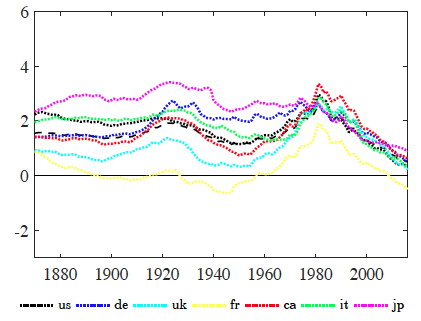
\includegraphics{Figures/delnegro12novfig4.png}
}

\end{center}
\caption{Substantial declines in `long run value' of \textit{real} rates in recent times, across many countries, Source: \href{https://voxeu.org/article/global-trends-interest-rates}{NY Fed}}
\end{figure}

\end{frame}

%-------------------------------------------------------

%-------------------------------------------------------

\begin{frame}{Real rates have declined to historically low levels}

The debate over falling real rates often refers to the long run `neutral' rate as $r^{\ast}$ or `r star'
\begin{itemize}
\item	From the reading list
	\begin{itemize}
	\item	Laubach and Williams (2015),
	\item	Williams (2018)
	\end{itemize}
\item	Also see \href{https://voxeu.org/article/global-trends-interest-rates}{here}, \href{https://voxeu.org/article/causes-and-consequences-persistently-low-interest-rates}{here} and \href{https://www.niesr.ac.uk/sites/default/files/publications/Box\%20A\%20-\%20Decline\%20interest\%20rates.pdf}{here}
\end{itemize}	

\vspace{2mm}
Connected to the broader debate on `secular stagnation'
\begin{itemize}
\item	Some argue US GDP trend growth $\downarrow$ from $3.5\%$ to $1.9\%$
\item	Collection of essays \href{https://voxeu.org/content/secular-stagnation-facts-causes-and-cures}{here} (if you're interested)
\end{itemize}

\end{frame}

%-------------------------------------------------------

%-------------------------------------------------------
	
\begin{frame}{Falling nominal rates}

Recall Fisher equation $i_{t} = r_{t} + E_{t}[\pi_{t+1}]$
\begin{itemize}
\item	If inflation expectations are stable (or falling), $i_{t}$ will fall with $r_{t}$
\end{itemize}

\vspace{2mm}
A shock (say, negative innovation to $Z_{t}$) may require $r_{t}$ to be lowered as part of optimal policy
\begin{itemize}
\item	$r^{\ast} \downarrow$ problematic if $\pi$ too low for $r_{t}<0$ given $i_{t}\geq0$
\item	Arises if desired $r_{t}$ (implied by a Taylor rule, perhaps) $< -E_{t}[\pi_{t+1}]$
\end{itemize}

\vspace{2mm}
Why is it typically thought $i_{t}\geq0$?
\begin{itemize}
\item	Option to hold cash, which earns a $0$ net nominal return
\item	Zero is better than negative!
%\item	Though we have seen moderately negative rates in some European countries recently - active debaet\ldots
\end{itemize}

\vspace{2mm}
During Great Recession and afterwards, standard policy rules $\Rightarrow$ negative nominal rates were necessary
\begin{itemize}
\item	U.S. and other countries hit the \emph{Zero Lower Bound}
\end{itemize}

\end{frame}

%-------------------------------------------------------

%-------------------------------------------------------
	
\begin{frame}{Nominal rates have declined to historically low levels}

\begin{figure}
\begin{center}

\resizebox{0.65\textwidth}{!}{%
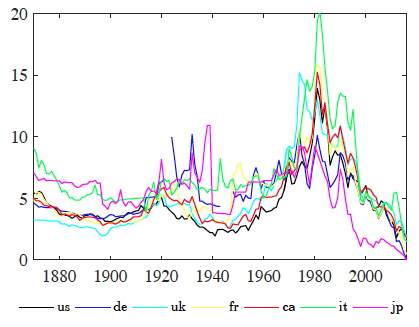
\includegraphics{Figures/delnegro12novfig1.png}
}

\end{center}
\caption{Substantial declines in rates in recent times, across many countries, Source: \href{https://voxeu.org/article/global-trends-interest-rates}{NY Fed} and \href{http://www.macrohistory.net/data}{Jorda \textit{et al's} Macrohistory Database}}
\end{figure}

\end{frame}

%-------------------------------------------------------

%-------------------------------------------------------
	
\begin{frame}{ZLB - short rates constrained}

\begin{figure}
\begin{center}

\resizebox{0.65\textwidth}{!}{%
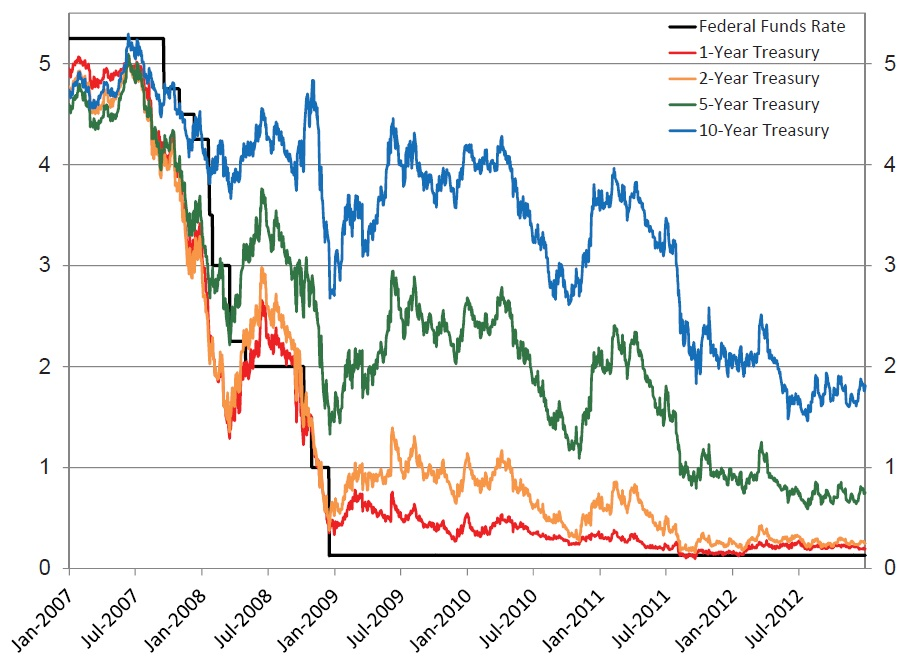
\includegraphics{Figures/williams_swanson_ZLB_frbsf_wp_long_term_rates.jpg}
}

\end{center}
\caption{Fed funds rate target and 1-, 2-, 5- and 10-year zero-coupon Treasury yields. Source: Federal Reserve Board and the Gurkaynak, Sack and Wright (2007) online dataset}
\end{figure}

\end{frame}

%-------------------------------------------------------

%-------------------------------------------------------
	
\begin{frame}{ZLB - inflation (and expectations?) declining}

\begin{figure}
\begin{center}

\resizebox{0.75\textwidth}{!}{%
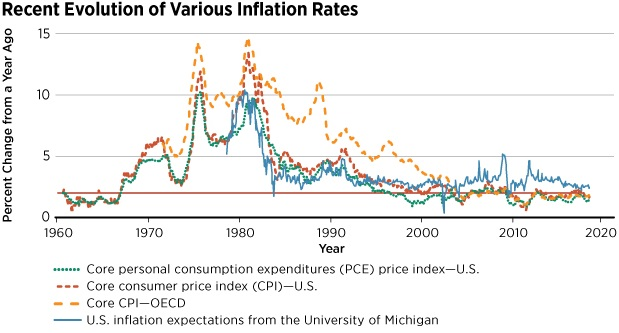
\includegraphics{Figures/Sanchez_fig1.jpg}
}

\end{center}
\caption{Declining U.S. inflation rate and expectations (red line is Fed's inflation target of $2\%$, Source: \href{https://www.stlouisfed.org/publications/regional-economist/first-quarter-2018/why-inflation-so-low}{St. Louis Fed}}
\end{figure}

\end{frame}

%-------------------------------------------------------

%-------------------------------------------------------
	
\begin{frame}{ZLB - short rates constrained}

To re-emphasize\ldots
\begin{itemize}
\item	Suppose $E_{t}[\pi_{t+1}]\leq \pi_{low}$
\item	Then real rate is constrained: $r_{t}\geq -\pi_{low}$ (as $i_{t}\geq 0$)
\item	Imagine $\pi_{low}=0$ then cannot set real rate negative (which has frequently helped stimulate the economy in other recessions)
\end{itemize}

\vspace{2mm}
Intuitively, monetary policy remains tight when it should be loose
\begin{itemize}
\item	CB cannot implement the responses in $r_{t}$ that we discussed earlier
\item	Theoretical possibility of being trapped in a deflationary spiral
\item	Scary - scan sections of \href{http://web.mit.edu/krugman/www/spiral.html}{Krugman reading} (up to and including `Adding the liquidity trap')
\end{itemize}

\vspace{2mm}
Useful readings for this topic
\begin{itemize}
\item	\href{https://www.brookings.edu/wp-content/uploads/2017/03/5_kileyroberts.pdf}{Kiley and Roberts (2017)} - Some of this too difficult but read the early sections - it contains nice overviews
\item	\href{https://www.brookings.edu/blog/ben-bernanke/2017/04/12/how-big-a-problem-is-the-zero-lower-bound-on-interest-rates/}{Bernanke (2017, `How big a problem\ldots)'}
\end{itemize}

\end{frame}

%-------------------------------------------------------

%-------------------------------------------------------
	
\begin{frame}{Is there anything we can do?}

\begin{itemize}
\item	Yes, maybe
	\begin{itemize}
	\item	Ask the Japanese how hard it is, and the current Fed and ECB policymakers how they feel about the situation right now\ldots
	\item	A lot of discussion of \textit{possible} new operating frameworks for Fed (e.g. price level targeting)
	\item	See \href{https://www.brookings.edu/research/monetary-policy-in-a-new-era/}{Bernanke (2017, `Mon. pol. in a new era')} and \href{https://www.brookings.edu/blog/up-front/2018/09/14/comments-on-monetary-policy-at-the-effective-lower-bound/}{Yellen (2018)}
	\end{itemize}
\vspace{2mm}
\item	Various possibilities - a few are\ldots
	\begin{itemize}
	\item	Forward guidance
	\item	QE
	\item	Fiscal expansion
	\item	Raise inflation target
	\item	Introduce price-level targeting
	\end{itemize}
\end{itemize}

\end{frame}

%-------------------------------------------------------

%-------------------------------------------------------
	
\begin{frame}{Forward guidance}

Setting ZLB aside, recall our DIS equation from the NK lecture
\begin{eqnarray*}
\tilde{y}_{t} &=& E_{t} \left[ \tilde{y}_{t+1} \right] - \frac{1}{\sigma} \left(i_{t} - E_{t}\left[ \pi_{t+1} \right]  - r^{n}_{t} \right) \label{eqn:dyn_IS} \\
&=& -\frac{1}{\sigma} \sum\limits_{k=0}^{\infty} E_{t}[ r_{t+k}  - r^{n}_{t+k} ] \nonumber \\
&=& -\frac{1}{\sigma} \sum\limits_{k=0}^{\infty} E_{t}[ i_{t+k} -  (r^{n}_{t+k} + \pi_{t+k+1}) ] \nonumber
\end{eqnarray*}
where we used the Fisher equation and $E_{t}[E_{t+k}[\pi_{t+k+1}]]= E_{t}[\pi_{t+k+1}]$

\vspace{2mm}
Current output gap reflects current and expected values of $i_{t}$, $\pi_{t}$ $r^{n}_{t}$
\begin{itemize}
\item	Assume, as \textit{in our simple NK model}, $y^{n}_{t}$ is independent of $v_{t}$ and $z_{t}$
\item	If the C.B. sets \textit{or is expected} to set $i_{t}$ in a particular way then it may influence the output gap - also may be able to influence $E_{t}[\pi_{t+k}]$
\end{itemize}

\end{frame}

%-------------------------------------------------------

%-------------------------------------------------------
	
\begin{frame}{Williams and Swanson 2013 - Long rate sensitivity to news}

\begin{figure}
\begin{center}

\resizebox{0.35\textwidth}{!}{%
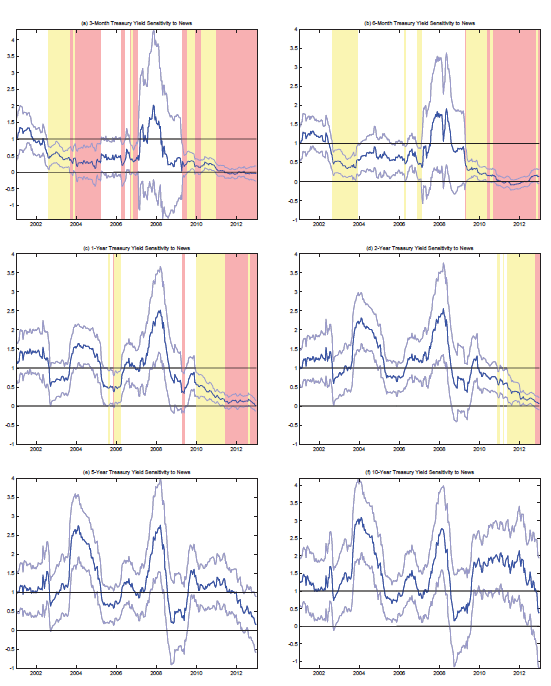
\includegraphics{Figures/williams_swanson_sensitive_guide_frbsf_wp_long_term_rates.png}
}

\end{center}
\caption{Sensitivity of Treasury yields to news (3-Mo, 6-Mo, 1-Y, 2-Y, 5-Y, 10-Y), Red and yellow indicate periods of insensitivitiy. Source: \href{https://pubs.aeaweb.org/doi/pdfplus/10.1257/aer.104.10.3154}{Swanson and Williams (2014)}}
\end{figure}

\end{frame}

%-------------------------------------------------------

%-------------------------------------------------------
	
\begin{frame}{Forward guidance}

\begin{equation*}
\tilde{y}_{t} = -\frac{1}{\sigma} \sum\limits_{k=0}^{\infty} E_{t}[ i_{t+k} -  (r^{n}_{t+k} + \pi_{t+k+1}) ]
\end{equation*}
\begin{itemize}
\item	Guidance about how rates will behave after period of ZLB can be influential if it is \textbf{credible}
\item	If CB can affect expectations of $i_{t+j}$ and $\pi_{t+j}$ \emph{in the future} then can influence economy even if currently at ZLB
	\begin{itemize}
	\item	See \textit{introductions} of papers on reading list and \href{https://www.frbsf.org/economic-research/files/SecretsShort-NBER-ch6-2008.pdf}{this classic}
	\item	Also see \href{https://uk.reuters.com/article/us-usa-fed-williams/feds-williams-makes-case-for-lower-for-longer-rates-idUKKCN1S91OE}{here}, \href{https://www.newyorkfed.org/newsevents/speeches/2019/wil190718}{here} and \href{https://www.brookings.edu/blog/up-front/2018/09/14/comments-on-monetary-policy-at-the-effective-lower-bound/}{here}
	\end{itemize}
\item	Some channels:
	\begin{itemize}
	\item	Many borrowing rates (e.g. mortgages) are at longer maturities and perhaps can be influenced
	\item	Might enhance confidence
	\item	Could induce depreciation in exchange rate - stimulating exports (and maybe raising inflation)
	\end{itemize}
\item	But\ldots theory is subtle/debatable
\end{itemize}

\end{frame}

%-------------------------------------------------------

%-------------------------------------------------------
	
\begin{frame}{Fed date-based guidance - powerful effect in 2011}

\begin{figure}
\begin{center}

\resizebox{0.35\textwidth}{!}{%
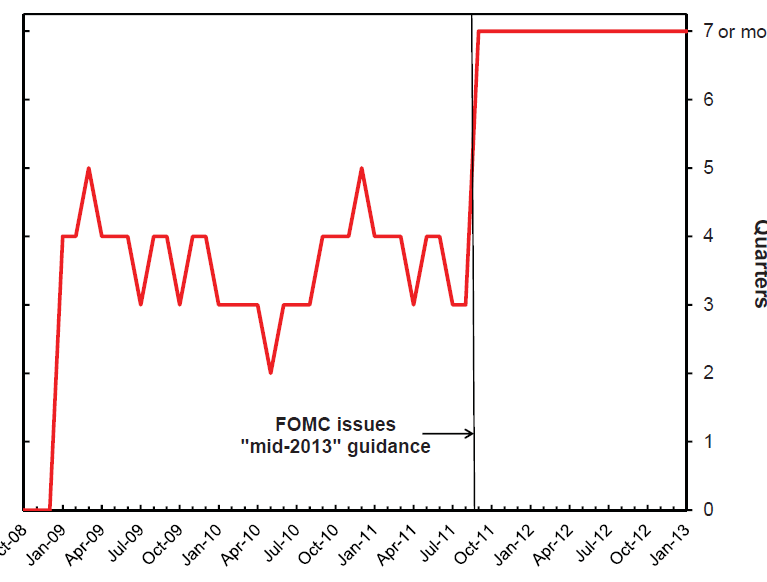
\includegraphics{Figures/williams_swanson_2013_guide_frbsf_wp_long_term_rates.png}
}

\end{center}
\caption{Effect of explicit date-based forward guidance (implemented in mid 201) on expected number of quarters until `lift-off' from ZLB, Source: Blue Chip and \href{https://pubs.aeaweb.org/doi/pdfplus/10.1257/aer.104.10.3154}{Swanson and Williams (2014)}}
\end{figure}

\begin{itemize}
\item	In 2011, economic conditions, \emph{`likely to warrant exceptionally low levels for the federal funds rate at least through mid-2013'}
\item	Compare with, less explicit, `indications that rates were likely to stay low \emph{`for some time'}
\end{itemize}

\end{frame}

%-------------------------------------------------------

%-------------------------------------------------------
	
\begin{frame}{Raising (or stabilizing?) inflation expectations}

Some people have suggested revisiting the Fed's interpretation of the `price stability' aspect of its \href{https://www.chicagofed.org/research/dual-mandate/dual-mandate}{`dual mandate'}
\begin{itemize}
\item	Fed pursues a $2\%$ inflation target, which was asserted before people fully grasped the scale of $r^{\ast}\downarrow$
\item	Some people think the decline has been from $3.5\%$ to approx $0,5\%$
\item	Thus, in `steady state' the nominal rate probably now sits around $2.5\%-3.0\%$, rather than $5.5\%$ as previously
\item	Means that there is less room to cut in a recession (before hitting ZLB)
\end{itemize}

\vspace{2mm}
See \href{https://www.jstor.org/stable/2138238}{Bernanke and Mishkin (1997)} on reading list or \href{https://www.imf.org/external/pubs/ft/fandd/basics/target.htm}{here} for more on inflation targeting
\begin{itemize}
\item	Recall also our conventional monetary policy price stability discussion
\item	Due to quality improvements etc. $2.0\%$ rather than literally $0\%$ is interpreted as price stability
\end{itemize}

\end{frame}

%-------------------------------------------------------

%-------------------------------------------------------
	
\begin{frame}{Raising (or stabilizing?) inflation expectations}

One option discussed is to raise the inflation target (see chapter 1 \href{https://www.niesr.ac.uk/sites/default/files/publications/Renewing\%20our\%20Monetary\%20Vows\%20text.pdf}{here})
\begin{itemize}
\item	What seems increasingly to be proposed instead is `price level targeting'
\item	See \href{https://www.jstor.org/stable/2601112}{Svensson (1999)}, \href{https://www.brookings.edu/research/monetary-policy-in-a-new-era/}{Bernanke (2017)} (easier) and \href{https://www.investopedia.com/terms/p/price_level_targeting.asp}{Investopedia} (easiest)
\end{itemize}

\vspace{2mm}
Main difference between price level and inflation targeting is that price level targeting implies a promise to adjust for past inflation misses
\begin{itemize}
\item	Under inflation targeting: If you suffer a few periods of sub-target inflation, that doesn't change the aim to hit target inflation from today onwards
\item	Under price-level targeting: If you suffer a few periods of sub-target inflation, you aim for higher than target inflation until you're back on the initial price path
\end{itemize}

\end{frame}

%-------------------------------------------------------

%-------------------------------------------------------
	
\begin{frame}{Raising (or stabilizing?) inflation expectations}

\begin{figure}
\begin{center}

\resizebox{0.50\textwidth}{!}{%
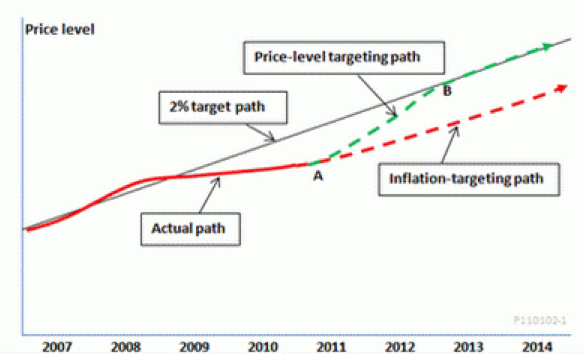
\includegraphics{Figures/price-level-target11.png}
}

\end{center}
\caption{Price and inflation behavior under inflation targeting and price level targeting, Source: \href{https://econfix.wordpress.com/2011/07/02/price-level-targeting-and-inflation-targeting-part-1-the-theory/}{Econfix}}
\end{figure}

\begin{itemize}
\item	So? Because of ZLB we are particularly concerned with the level of inflation and even downward drift in inflation expectations
\item	PLT `could' be a credible way of promising higher inflation in the near term, helping to lower real rates now, thus stimulating the economy
\end{itemize}

\end{frame}

%-------------------------------------------------------

%-------------------------------------------------------
	
\begin{frame}{Quantitative Easing}

\begin{figure}
\begin{center}

\resizebox{0.55\textwidth}{!}{%
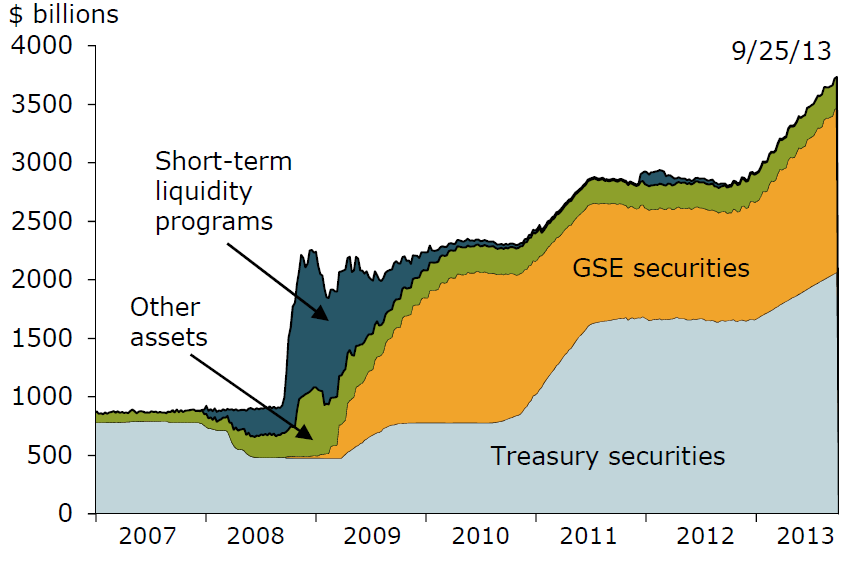
\includegraphics{Figures/williams_el_fed_balance_sheet.png}
}

\end{center}
\caption{Federal Reserve asset holdings, Source: Federal Reserve Board.}
\end{figure}

Fed massively expanded its balance sheets to purchase assets
\begin{itemize}
\item	Initially some liquidity programs - but most importantly QE
\item	Nice readable review \href{https://www.frbsf.org/economic-research/publications/economic-letter/2018/december/review-of-unconventional-monetary-policy/}{here} with good bibliography if you're interested
\end{itemize}

\end{frame}

%-------------------------------------------------------

%-------------------------------------------------------
	
\begin{frame}{Quantitative Easing}

QE1 (December 2008)
	\begin{itemize}
	\item	$\$600bn$ of \href{https://www.investopedia.com/terms/a/agency-mbs-purchase.asp}{agency MBS} and debt - initially sterilized
	\item	Later $\$750bn$ more + $\$300bn$ Treasuries - not sterilized (QE up and running)
	\end{itemize}
\vspace{3mm}
QE2 (November 2010)
	\begin{itemize}
	\item	$\$600bn$ of long-dated Treasuries ($BS\uparrow$)
	\end{itemize}

\end{frame}

%-------------------------------------------------------

%-------------------------------------------------------
	
\begin{frame}{Quantitative Easing}

Operation Twist (2011)
	\begin{itemize}
	\item	Purchase $\$400bn$ bonds with maturities $6$ to $30$ years, using proceeds from selling bonds with maturities less than $3$ years
	\item	Limited impact on size of balance sheet - changing composition
	\item	Lengthened average maturity and `removed duration' from market
	\item	Later extended with further $\$267bn$
	\item	Eventually ran out of short dated to sell
	\end{itemize}
\vspace{2mm}
QE3 (2012)
	\begin{itemize}
	\item	Open ended commitment to purchase $\$40bn$ agency MBS until labor market improved
	\item	Later added up $\$45bn$ long dated Treasury purchases per month
	\end{itemize}

\end{frame}

%-------------------------------------------------------

%-------------------------------------------------------
	
\begin{frame}{Balance sheet decomposition - asset class}

\begin{figure}
\begin{center}

\resizebox{0.80\textwidth}{!}{%
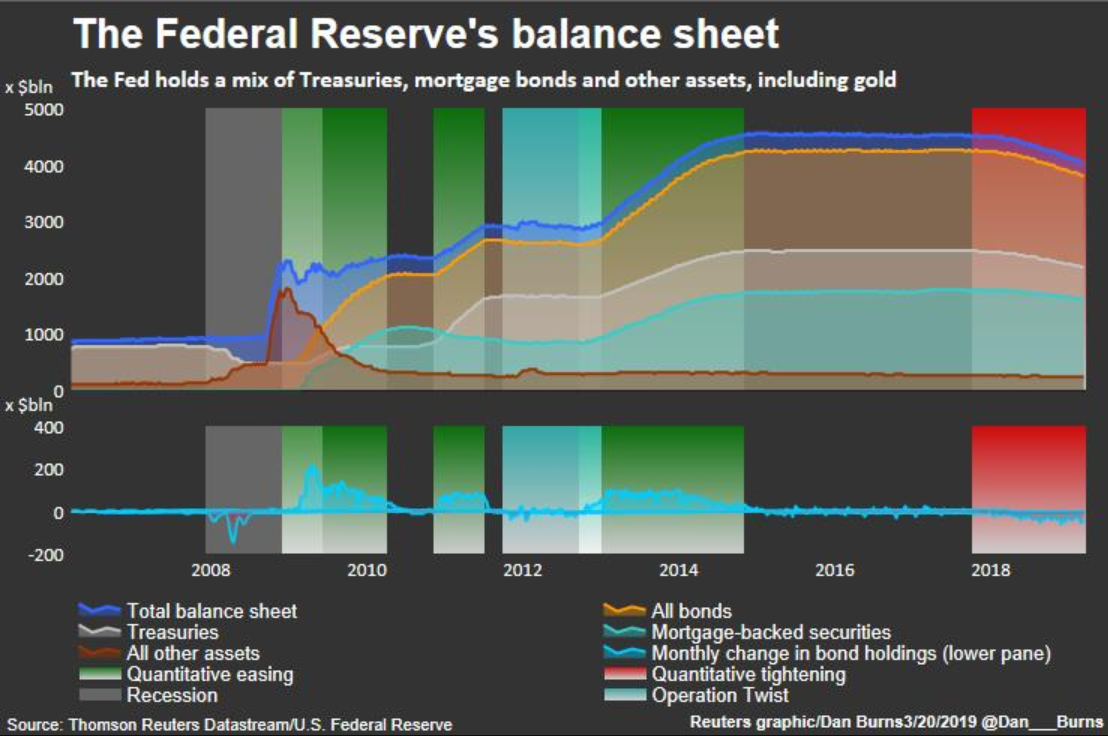
\includegraphics{Figures/fed_bs_decomp.png}
}

\end{center}
\end{figure}

\end{frame}

%-------------------------------------------------------

%-------------------------------------------------------
	
\begin{frame}{Balance sheet decomposition - maturity}

\begin{figure}
\begin{center}

\resizebox{0.80\textwidth}{!}{%
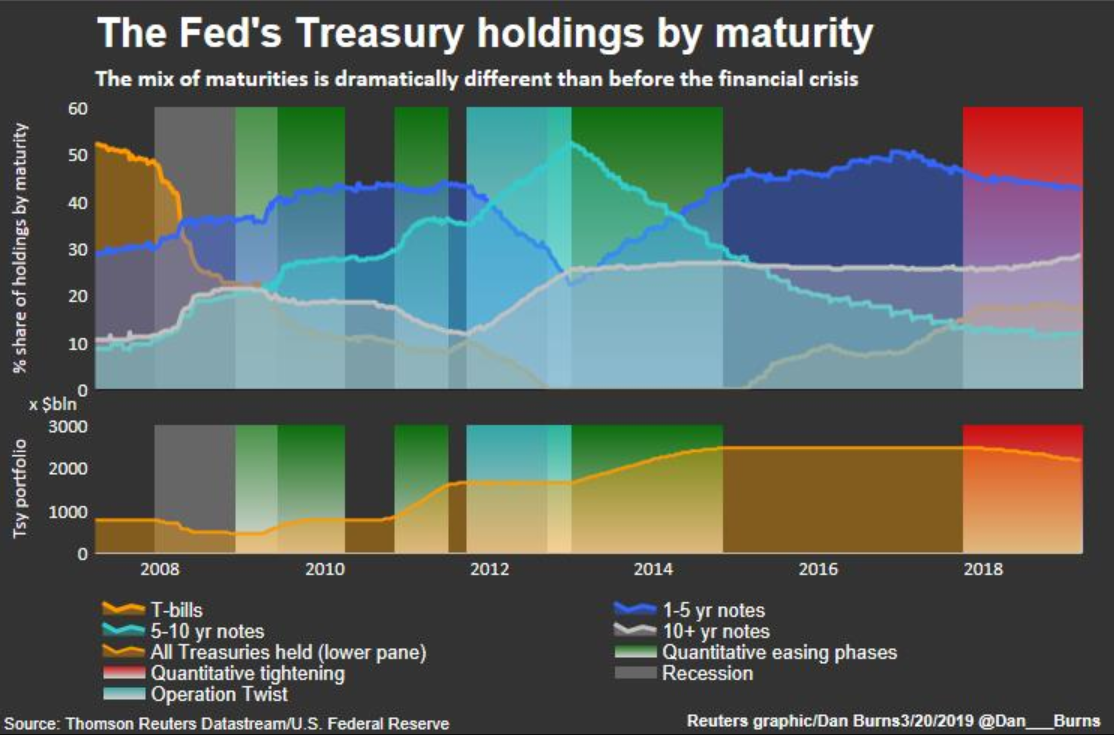
\includegraphics{Figures/fed_bs_decomp_maturity.png}
}

\end{center}
\end{figure}

\end{frame}

%-------------------------------------------------------

%-------------------------------------------------------
	
\begin{frame}{Channels}

Main intended channels
	\begin{itemize}
	\item	Drive down long rates (similar aim to FG) - paper \href{https://academic.oup.com/ej/article/122/564/F385/5079473}{here} if interested
	\item	Induce substitution into other - riskier - assets (e.g. mortgages, C\&I)
	\item	Stimulate stock market (aiding wealth and confidence)
	\item	See Gagnon papers,, D'Amico and Carpenter, plus \href{https://www.piie.com/system/files/documents/pb18-19.pdf}{this nice overview}
	\end{itemize}
\vspace{2mm}
Theoretical basis somewhat unclear (still)
	\begin{itemize}
	\item	But empirically, rates did seem to drop - at least around impact
	\item	VAR analysis and other approaches also suggest effect on economy
	\end{itemize}
\vspace{2mm}
Possible additional channels
	\begin{itemize}
	\item	Conveying commitment or signaling future $i_{t}^{e}$ policy - see \href{https://www.ijcb.org/journal/ijcb14q3a7.htm}{here}
	\item	Weakening exchange rate (though not primary aim)
	\item	Solidifying bank balance sheets (from rising asset prices)
	\end{itemize}

\end{frame}

%-------------------------------------------------------

%-------------------------------------------------------
	
\begin{frame}{Stimulating risk assets? Dow Jones}

\begin{figure}
\begin{center}

\resizebox{0.80\textwidth}{!}{%
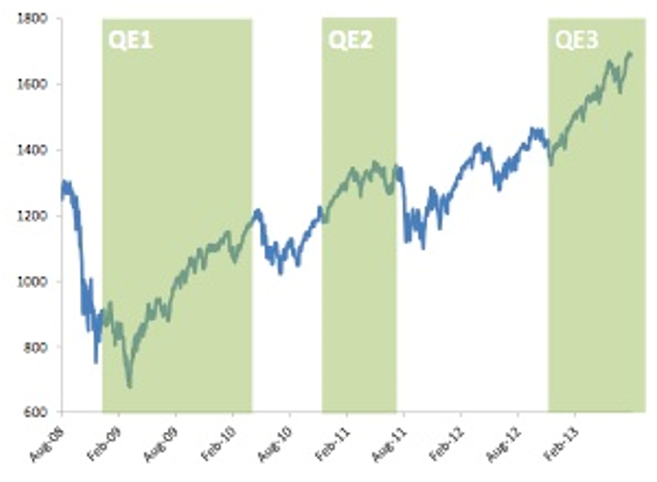
\includegraphics{Figures/Dow_Jones_QE123.png}
}

\end{center}
\end{figure}

\end{frame}

%-------------------------------------------------------

%-------------------------------------------------------
	
\begin{frame}{Fiscal policy?}

Big increase in `G' can `shift' the IS curve far to the `right'
\begin{itemize}
\item	Effectively a large demand shock that raises the $r_{t}$ that should be sought by the CB
\item	Blasts the economy out of the ZLB
\end{itemize}

\vspace{2mm}
Is it that easy?
	\begin{itemize}
	\item	Not necessarily
	\item	Ricardian equivalence and expectations of future taxes (if spending is deficit financed)
	\item	May mean a loss of confidence or leave expected effect on permanent income $\approx$ zero
	\item	Countries already in a bad fiscal position (esp. if they've bailed out banks) may not be `allowed' by the markets to borrow to fund spending - and raising taxes is difficult in recession
	\end{itemize}
	
\end{frame}